\documentclass[11pt]{amsbook}

\usepackage{../HBSuerDemir}	% ------------------------


\begin{document}

% ++++++++++++++++++++++++++++++++++++++
\hPage{b1p2/295}
% ++++++++++++++++++++++++++++++++++++++

% =======================================
    \\Evaluating H, $\Delta$ and T for ($1$), ($1'$), ($1''$) we have
    
    \[
    H= 2+1 = 3 ,\quad  \Delta = 3-8 = -5 , \quad
    T =  \left| \begin{array}{ccc}
        4 & \sqrt[]3 & -1 \\
        \sqrt[]3 & 2 & 1 \\
        -1 & 1 & -4 \end{array} \right|  = -2 (13 + \sqrt[]3)
    \] 

    \[
    H'= 2+1 = 3 ,\quad  \Delta ' = 3-8 = -5 , \quad
    T' =  \left| \begin{array}{ccc}
        4 & \sqrt[]3 & 0 \\
        \sqrt[]3 & 1 & 0 \\
        0 & 0 & 2(13+\sqrt[]3) \end{array} \right|  = -2 (13 + \sqrt[]3)
    \] 

    \[
    H''= \frac{5}{2}+ \frac{1}{2} = 3 ,\quad  \Delta '' = 0-4.\frac{5}{2} . \frac{1}{2} = -5 , \quad
    T'' =  \left| \begin{array}{ccc}
        5 & 0 & 0 \\
        0 & 1 & 0 \\
        0 & 0 & -\frac{2}{5}(13 + \sqrt[]3) \end{array} \right|  = -2 (13 + \sqrt[]3)
    \] 

    Hence $H$ = $H'$ = $H"$, $\Delta$ = $\Delta '$ = $\Delta ''$ and $T$ = $T'$ = $T"$



% =======================================
\subsection*{E. DETERMINANTAL EQUATIONS OF SECOND DEGREE CURVES:}

    \\A second degree curve has the equation
    \[
    f(x,y) = Ax^2 + Bxy + Cy^2 + Dx + Ey + F = 0, \quad (A^2 + B^2 + C^2 \neq 0) \quad (1)
    \]
    where at least one of A, B, C is not zero. Dividing every term by that non zero coefficient, the equation will involve in general 5 parameters. So a second degree curve is completely determined, in general, by five conditions.
    
    \\ Let the equation of a second degree curve passing through the five distinct points \(A_i(x_i , y_i), \quad i = 1 , 2, 3, 4 ,5\) be determined. Since (1) is satisfied by a general point \(P (x, y)\) and \(A_i(x_i , y_i), \quad i = 1 ,\quad ... \quad,5\) we have six homogeneous linear equations (corresponding to given five conditions):
    \[
    f (x, y) = 0, f(x_1, y_1) = 0, \quad ... \quad , f(x_5, y_5) = 0
    \] 
    in the six unknown coefficients A, B, C, D, E, F. The homogeneous system to have a nontrivial solution it is necessary that the determinant of the coefficients of unknowns vanish.

% =======================================================
\end{document}  

%==== templates ====

%==== environments ====

%\begin{figure}[htb]
%	\centering
%	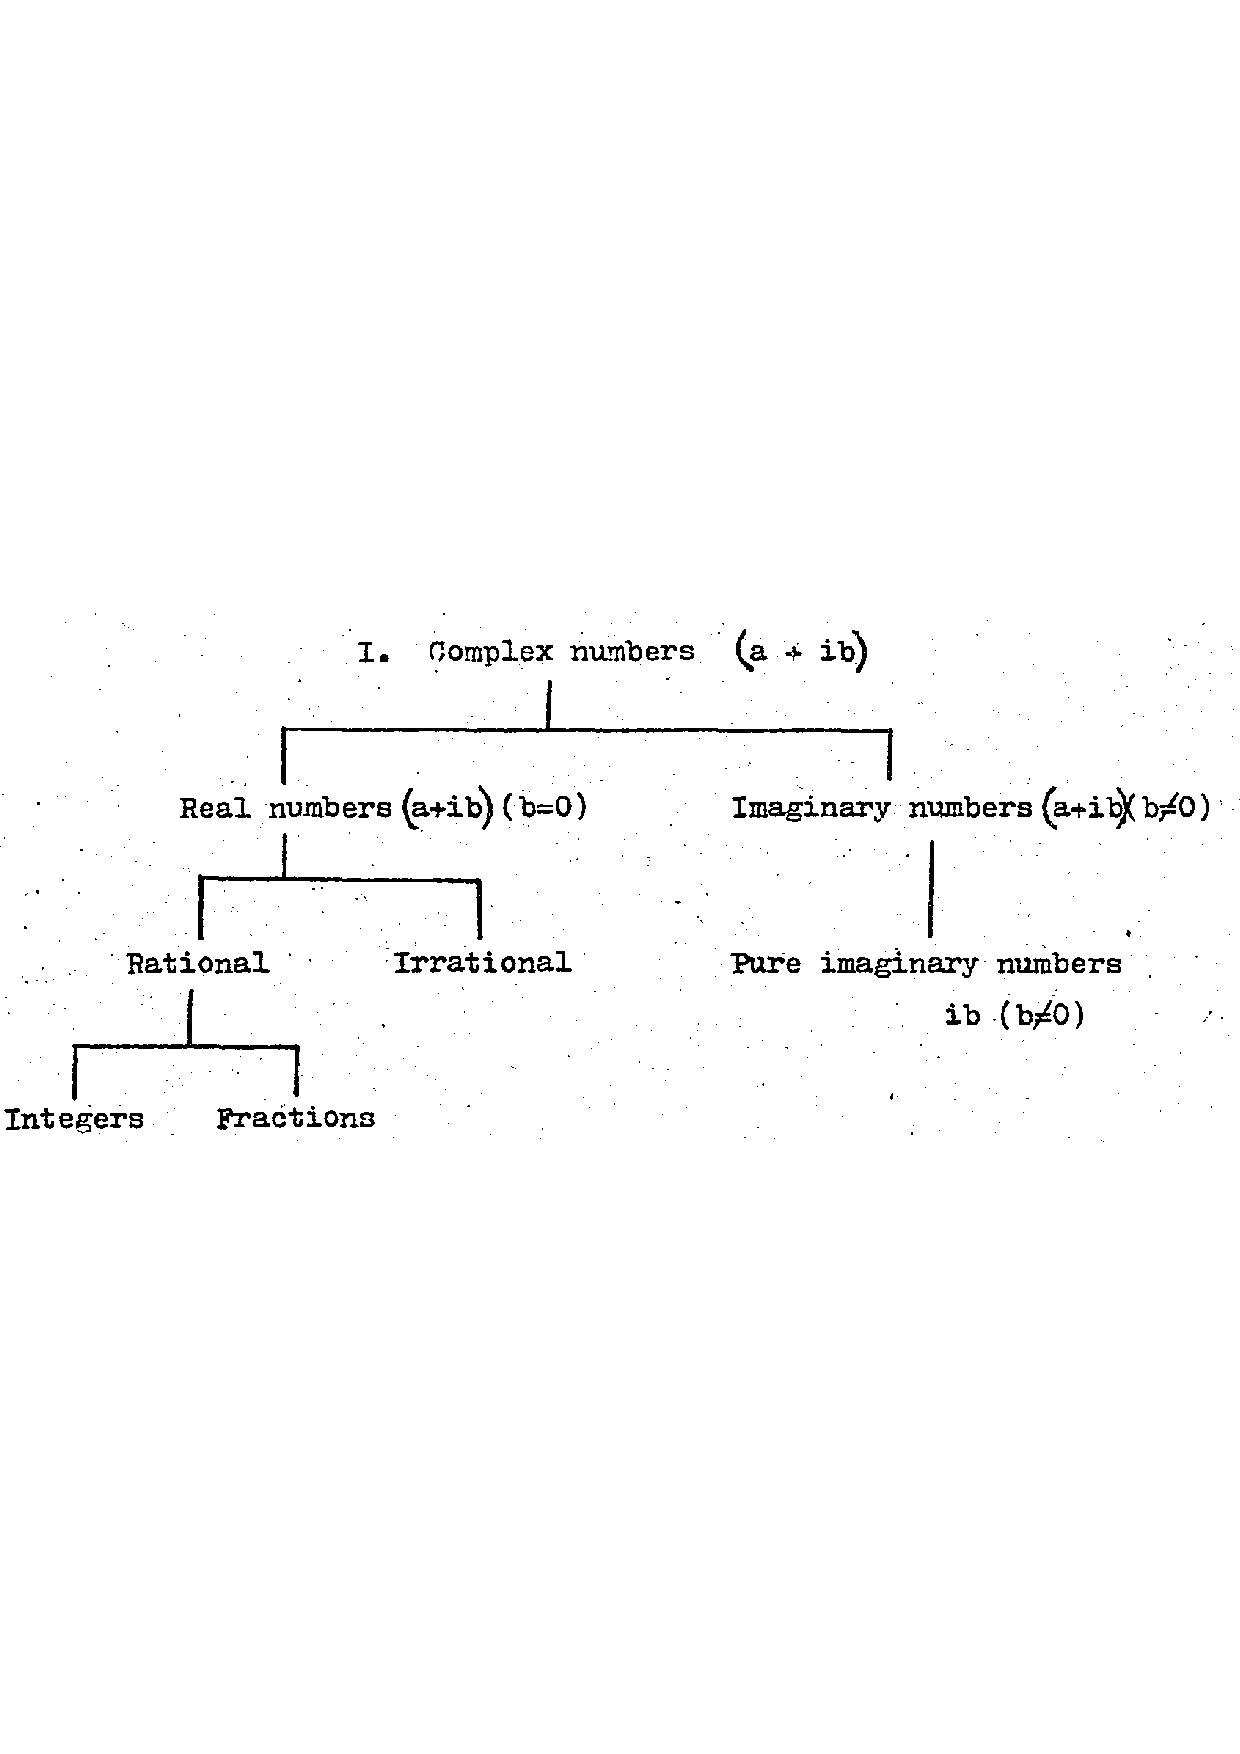
\includegraphics[width=0.9\textwidth]{images/SD-1-1p15A}
%	\caption{Classification of complex numbers}
%	\label{fig:classificationOfComplexNumbersA}
%\end{figure}

%\begin{center}
%\begin{tabular}{cc}
%\end{tabular}
%\end{center}

%\begin{exmp}
%\begin{hSolution}
%\end{hSolution}
%\end{exmp}

%\begin{hEnumerateAlpha}
%\end{hEnumerateAlpha}

%\begin{hEnumerateRoman}
%\end{hEnumerateRoman}

%$
%\begin{bmatrix}
%\end{bmatrix}
%$

%\frac{aaaa}{bbb}
%\frac{a_{n}}{b_{n}}
%\left( aaaa \right)
%\Longrightarrow

%\begin{multicols}{2}
%	bb
%\columnbreak
%	aa
%\end{multicols}